This chapter describes the developed predictive display. The final results only requires a few lines of code and can be applied to most ROVs. In the coming explanation a very simple and limited ROV is considered, but section \ref{expand} describes how the principle can be expanded to more complicated configurations.

\section{Robot configuration} \label{chp31}
 
To explain how the predictive display (PD) works, let us consider the self balancing two wheeled robot depicted in \figref{twoWheeled}. The upper part of the figure shows the robot from above with two objects in front of it, a black cube and a gray barrel. The ROV is drawn at time equal to $t=0$ and $t=\Delta t$. The bottom part of the image depicts the viewport of the onboard camera mounted to the ROV.


\begin{figure}[h!]    
    \centering           
    \def\svgwidth{.75\columnwidth}
    \input{img/twoWheeled.pdf_tex}
    \caption{Two wheeled robot before and after counter clockwise rotation.}
    \label{twoWheeled}
\end{figure}


It has a forward facing camera with a FOV of $\phi$ degrees. The camera captures a video feed with a resolution of $R_h$ pixels horizontally. Its center of rotation is located in the vector $z$ pointing out of the paper. It is able to rotate with an angular velocity of $\omega$ deg/sec around its center of rotation $z$.

Let us first consider a situation without delay and where the ROV can only be given two commands, to turn either left or right. The commands are given by pressing one of two buttons, not by a joystick with variable output. If the operator hold's down the \emph{left} button for a period of $\Delta t$ seconds, the ROV would make an angular rotation of $\omega \cdot \Delta t = \Delta \theta$ degrees. This is depicted in the right side of \figref{twoWheeled}.

In the viewport, the cube and barrel would move to the right as the ROV turned left. These objects has moved a finite number of pixels horizontally $\Delta P_h$, which can be calculated by Equation \ref{deltaph}. It is simply the ratio between the angular rotation and the FOV, times the pixel screen width. By substituting in the expression for angular rotation, Equation \ref{pixelturnrate} is obtained. Here $\eta$ is used to denote the \textit{pixel turn rate}; the pixel rate at which objects in the video moves left or right when the operator turns the ROV.

\vspace{7mm}
\begin{equation}\label{deltaph}
\Delta P_h = \frac{\Delta \theta}{\phi}\cdot R_h
\end{equation}
\vspace{7mm}
\begin{equation}\label{pixelturnrate}
\Delta P_h = \left ( R_h\frac{\omega }{\phi} \right )\Delta t = \eta \cdot  \Delta t
\end{equation}
\vspace{0mm}

$\eta$ is a constant and depending on the screen resolution, camera FOV and the angular velocity of the ROV. By multiplying this factor by the amount of time the operator holds down the left or right button, the number of pixels the objects in the frame should move is obtained.

\section{Predictive visualization}

Let us now consider a situation where there is a $t_d$ seconds delay from when the commands are given by the operator, to the changes can be seen in the video feed. This is the \emph{total perceived delay} described in the introduction, section \ref{timeDelay}. For simplicity, let us also consider a situation where $\Delta t < t_d$.

\figref{movie} shows a representation of what the video feed would look like as the above maneuver was performed. It shows the situation in three different scenarios. First no delay, secondly with delay and third with the PD implemented using the delayed video. The outer rectangle shows the limitations of the monitor, while the inner rectangle is the video feed itself.

\begin{figure}[h!]    
    \centering           
    \def\svgwidth{.8\columnwidth}
    \input{img/movie.pdf_tex}
    \caption{Operator view. Outer box total screen size, inner box video feed.}
    \label{movie}
\end{figure}

\figref{timePlot} plots the visible angular rotation $\alpha$ for the no delay display and the delayed display as a function of time. For the no delay display, visible angular rotation is equal to ROV angular rotation $\alpha = \theta$. In addition, the horizontal image pixel displacement $P_h$ is plotted with the same time axis.

The PD works by moving the video feed on the operator screen the opposite way of what the ROV is moving. The amount of pixels the video $P_h$ is moved is calculated by Equation \ref{pixelturnrate}. In addition, the video is moved back (the same way as the ROV is moving) after $t_d$ seconds has passed. This makes the objects in the video feed appear in the correct position on the operator screen as if there were no delay. Note that the black box in \figref{movie} predictor display center column is in the correct position relative to the no delay display. This approach does however assume that the commands will be properly followed by the ROV. But since the prediction is merely an alteration to the last image received, the prediction errors are not cumulative.


\begin{figure}[h!]    
    \centering           
    \def\svgwidth{\columnwidth}
    \input{img/timePlot.pdf_tex}
    \caption{Visible angular rotation and horizontal image pixel displacement as a function of time.}
    \label{timePlot}
\end{figure}

\vspace{-3mm}
\section{Implementation}

Algorithm \ref{predictorAlg} shows the pseudocode for how this PD is implemented in practice. The horizontal pixel displacement $P_h$ is initialized as zero. Then, the \textsc{predictor display} function is called at a set interval $dt$. The rate of these calls should happen at least as fast as the frame rate of the video (fps). With a fps of 30, the interval should be $dt <= 1/30 \approx 33 ms$. The change in horizontal pixel displacement $\Delta P_h$ is then calculated from Equation \ref{pixelturnrate} and the interface is updated with the new $P_h$. In addition, an asynchronous call is done on the \textsc{move back} function so that the video is moved back to its original position after $t_d$ seconds has passed. It has to be an asynchronous call so that the main program is not blocked when the \textsc{move back} function is waiting.

\newgeometry{bmargin=0mm}
\begin{algorithm}
\caption{Predictive display}\label{predictorAlg}
\begin{algorithmic}[0]
\State $P_h$ = 0 \Comment{horizontal pixel displacement}
\State \Call{set interval}{predictor display, $d t$} \Comment{calls function at interval}
\State

\Function{predictor display}{}
\If{left}
	\State $\Delta P_h$ = $-\eta \cdot d t$ \Comment{equation \ref{pixelturnrate}}
\ElsIf{right}
	\State $\Delta P_h$ = $+\eta \cdot d t$ \Comment{equation \ref{pixelturnrate}}
\Else
	\State $\Delta P_h$ = 0
\EndIf

\State $P_h$ += $\Delta P_h$
\State \Call{update interface}{$P_h$}
\State \Call{move back}{$\Delta P_h$} \Comment{asynchronous call}

\EndFunction
\State

\Function{move back}{$\Delta P_h$}
\State wait $t_d$
\State $P_h$ -= $\Delta P_h$
\EndFunction

\end{algorithmic}
\end{algorithm}


\figref{predictorvis} shows the predictor display as it was implemented in the experiment, which is explained in chapter \ref{chpMethod}. It contains the video feed from the ROV, in addition to a red arrow to visualize the prediction. The operator has recently turned the ROV to the right, and as a result the video has moved to the left. The red arrow has not moved and works as an indication of where the ROV will be heading when the video feed has caught up with the time delay.

\begin{figure}[h!]
    \centering
    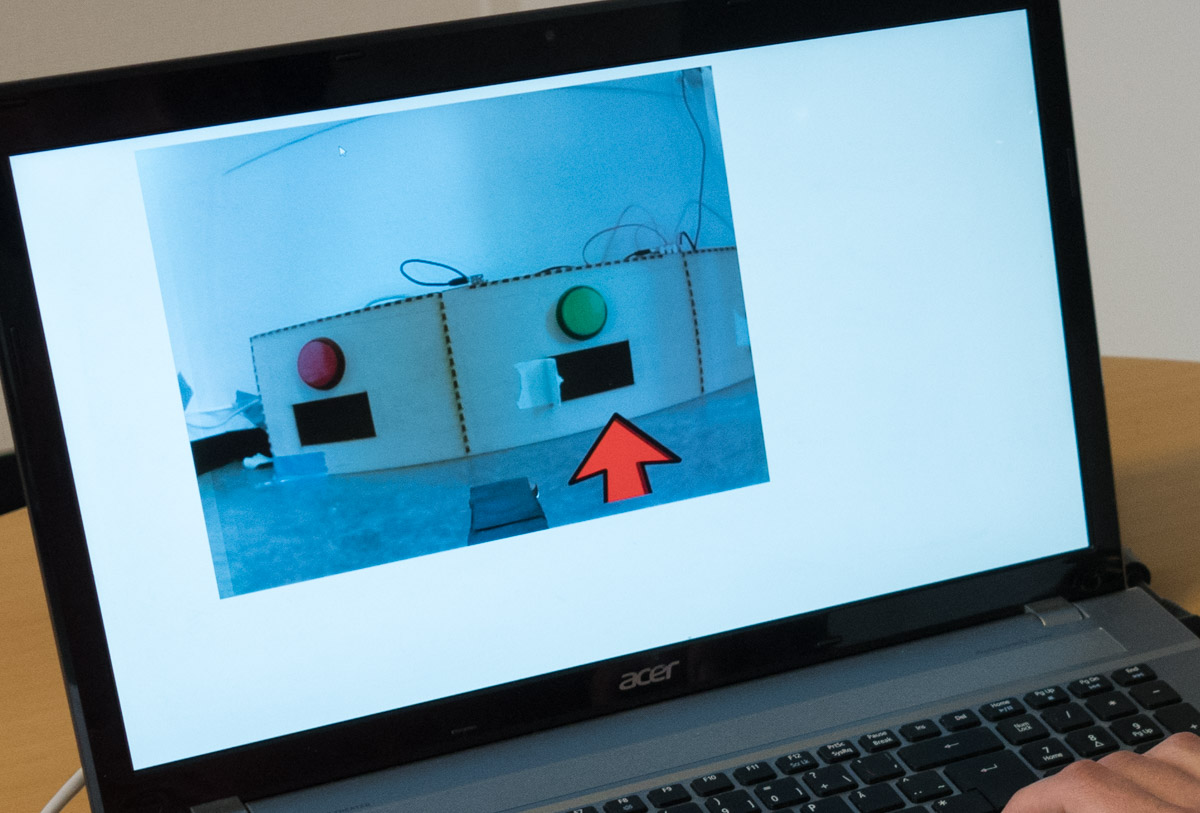
\includegraphics[width=0.7\textwidth]{setup-4}
    \caption{Predictor display visualization.}
    \label{predictorvis}
\end{figure}

\clearpage
\restoregeometry

The operator views the predictor screen through a web browser. The predictor algorithm is written in java script and the video feed is moved around by changing css margin properties. The code can viewed in its entirety in the appendix \hyperref[appPredict]{section C} on page \pageref{appPredict}, or online.\footnote{\url{https://github.com/trolllabs/eduROV/blob/master/examples/experiment/displays/predictive.js}}


\section{Extending and generalizing}\label{expand}

The pixel turn rate $\eta$ described in section \ref{chp31} was related to the rotation of the ROV. A similar constant can be found for the \emph{pixel scale rate}, which relates how the the video should be scaled when the ROV moves back and fourth. It's a bit more complicated since the apparent scaling of objects in the frame depends on how far away they are, but by using an average distance this can at least be approximated. The same approach as in Algorithm \ref{predictorAlg} can then be used for backward and forward motion to manipulate the scale of the video feed.

In the case of a varying magnitude of left, right, forward and backward movements. Such if the operator is using a joystick with variable output, the PD has to account for this. This can be achieved by applying an adjustment factor to the pixel turn/scale rate proportionate to the magnitude of the command.

The predictor display can then be applied to all moving ROVs. It's just a matter of finding the correct pixel turn/scale rate and adjustment factor's corresponding to how the ROV is moving. A submersible ROV would typically have a much lower pixel turn/scale rate because of water friction.

These rates and factors can be found by calculation using ROVs physics and screen resolution. But they can also be found using trial and error. For example, if the visual angular rotation is less than the actual angular rotation, increase the pixel turn rate until they match. In this way, the predictor display can be calibrated without knowing any of the ROVs physics. In this context, \emph{ROV physics} means how the ROV respond to operator input, how fast it moves and turns.